\documentclass[article,nojss]{jss}

%\VignetteIndexEntry{Tools for Exploring Multivariate Data: The Package ICS}
%\VignetteDepends{ICS,ICSNP,methods,mvtnorm,survey,pixmap,robustbase,MASS}
%\VignetteKeywords{clustering, discriminant analysis, independent components analysis, invariant coordinate selection, R, transformation-retransformation method}
%\VignettePackage{ICS} 

\usepackage{thumbpdf}
%% need no \usepackage{Sweave.sty}


\newcommand{\ave}{\mathrm{ave}}
\newcommand{\sgn}{\mathrm{sgn}}

\author{Klaus Nordhausen\\ University of Tampere \And
        Hannu Oja\\ University of Tampere \And
        David E. Tyler\\Rutgers, The State\\University of New Jersey}
\Plainauthor{Klaus Nordhausen, Hannu Oja, David E. Tyler}

\title{Tools for Exploring Multivariate Data: The Package \pkg{ICS}}
\Plaintitle{Tools for Exploring Multivariate Data: The Package ICS}
\Shorttitle{\pkg{ICS}: Tools for Exploring Multivariate Data}

\Abstract{
  This introduction to the \proglang{R}~package \pkg{ICS} is a (slightly)
  modified version of \cite{NordhausenOjaTyler2008}, published in the
  \emph{Journal of Statistical Software}.

  Invariant coordinate selection ({ICS}) has recently
  been introduced as a method for exploring multivariate data. It
  includes as a special case a method for recovering the unmixing
  matrix in independent components analysis ({ICA}). It also
  serves as a basis for classes of multivariate nonparametric tests, and as a tool in cluster analysis 
  or blind discrimination.
  The aim of this paper is to briefly explain the ({ICS}) method
  and to illustrate how various applications can be implemented using
  the \proglang{R}~package \pkg{ICS}. Several examples are used to
  show how the {ICS} method and \pkg{ICS} package can be used in
  analyzing a multivariate data set.
}

\Keywords{clustering, discriminant analysis, independent components analysis, invariant coordinate selection, \proglang{R}, transformation-retransformation method}
\Plainkeywords{clustering, discriminant analysis, independent components analysis, invariant coordinate selection, R, transformation-retransformation method}

\Volume{28}
\Issue{6}
\Month{November}
\Year{2008}
\Submitdate{2008-02-19}
\Acceptdate{2008-09-03}

\Address{
  Klaus Nordhausen\\
  Tampere School of Public Health\\
  University of Tampere\\
  33014 University of Tampere, Finland\\
  E-mail: \email{klaus.nordhausen@uta.fi}\\
  URL: \url{http://www.uta.fi/~klaus.nordhausen/}\\

  Hannu Oja\\
  Tampere School of Public Health\\
  University of Tampere\\
  33014 University of Tampere, Finland\\
  E-mail: \email{hannu.oja@uta.fi}\\
  URL: \url{http://www.uta.fi/~hannu.oja/}\\

  David E. Tyler\\
  Department of Statistics\\
  The State University of New Jersey\\
  Piscataway NJ 08854, USA\\
  E-mail: \email{dtyler@rci.rutgers.edu}\\
  URL: \url{http://www.rci.rutgers.edu/~dtyler/}
}

\begin{document}

\section{Introduction}

Multivariate data normally arise by collecting $p$ measurements on
$n$ individuals or experimental units. Such data can be displayed in
tables with each row representing one individual and each column
representing a particular measured variable. The resulting data
matrix $X$ is then $n \times p$, with the row vector $x_i \in \Re^p$
denoting the measurements taken on the $i$th individual or $i$th
experimental unit. Hence $X^\top = [ x_1^\top, \ldots, x_n^\top ]$. To be
consistent with the convention used in the programming language
\proglang{R}, all vectors are understood to be row vectors.

We begin by introducing some concepts which are used throughout the paper.
An affine transformation of a data vector $x_i$ is a transformation of the form
\[
x_i \rightarrow x_iA^\top +b,\qquad i=1,\ldots,n,
\]
or equivalently,
\[
X \rightarrow XA^\top +1_n^\top b,
\]
where $A$ is a nonsingular matrix of order $p$, $b \in \Re^p$, and
$1_n \in \Re^n$ denotes a vector consisting of all ones. Besides affine transformations and
linear transformations ($X \rightarrow XA^\top$ with $A$
nonsingular), other important classes of transformations are
orthogonal transformations ($X \rightarrow XU$ with $U^\top U=UU^\top =I_p$),
sign-change transformations ($X \rightarrow XJ$ where $J$ is a $p
\times p$ diagonal matrix with diagonal elements $\pm 1$), and
permutations ($X \rightarrow XP$ where $P$ is a $p \times p$
permutation matrix, i.e., one obtained by successively permuting
rows or columns of $I_p$). These transformations can also be applied
on the left-hand side of $X$, in which case $A$, $U$, $J$, and $P$
are matrices of order $n$ rather than of order $p$. Note, for
example,  that a right-sided sign-change transformation simply
results in a change of the sign of the $j$th variable if the $j$th
entry of $J$ is $-1$, whereas a left-sided permutation
transformation simply reorders the individual observations.

A fundamental multivariate data transformation method is the so-called `whitening' or `standardization'
of the data. This is given by
\[
X \rightarrow Z=(X-1_n^\top \bar{x})\COV(X)^{-\frac{1}{2}},
\]
where $\bar{x}= 1_nX/n = \sum_{i=1}^n x_i/n$ is the vector of the
column means of $X$ and $\COV(X)=
(X-1_n^\top \bar{x})^\top (X-1_n^\top \bar{x})/(n-1)$ is the sample covariance
matrix of the columns of $X$. The `whitened' data matrix $Z$ has its
mean at the origin $(\bar{z}=0)$, with all the variables being
standardized and uncorrelated with each other $(\COV(Z)=I_p)$.

This transformation, however, has several drawbacks. First, it is
not unique in the sense that it depends on the particular choice or
definition of the square-root matrix $\COV(X)^{\frac{1}{2}}$. Recall
that for a symmetric positive semi-definite matrix $V$, a square
root of $V$ is any matrix $C$ such that $CC^\top  = V$. Two common
choices for the square-root $C$ which are uniquely defined are the
lower triangular square-root and the symmetric positive definite
square-root. Second, even for a well defined square-root matrix, the
`whitening' transformation is not invariant under affine
transformations of the data. Rather, one has
\[
 XA^\top [\COV(XA^\top )]^{-\frac{1}{2}} = X[\COV(X)]^{-\frac{1}{2}}U,
\]
with $U=U(X,A)$ being an orthogonal matrix which is dependent on both $X$ and $A$. In other words, a `whitened' data matrix is only well defined
up to post multiplication by an orthogonal matrix.

Also, this `whitening' transformation is not very robust since both
the sample mean vector $\bar{x}$ and the sample covariance matrix
$\COV(X)$ are both highly non-robust statistics. In particular, just
one `bad' data point can greatly affect the standardization.  An
obvious remedy for the last problem is to simply replace those two
statistics by more robust ones. This gives a more general framework
for a whitening transformation, namely
\[
X \rightarrow Z=[X-1_n^\top T(X)]S(X)^{-\frac{1}{2}},
\]
where the statistic $T(X)$ is a multivariate location statistic and $S(X)$ is a scatter matrix.  Here, we say that
$T(X)$ is a location statistic if it is affine equivariant,
i.e., if
\[
T(XA^\top +1_n^\top  b)=T(X)A^\top +b
\]
for any nonsingular matrix $A$ of order $p$, and any $b \in \Re^p$. The matrix $S(X)$ is said to be a scatter matrix if it
is  affine equivariate in the following sense:
\[
S(XA^\top +1b)=AS(X)A^\top 
\]
with $A$ and $b$ as before. Such a statistic is sometimes referred to as being affine `covariant'. Choosing robust statistics
for $T(X)$ and $S(X)$ then yields a robustly whitened coordinate system. This new coordinate system though is still not invariant
under affine transformations of the original data matrix.

Besides whitening, there are other methods one can use to linearly transform a multivariate data set to a new coordinate system,
such as those arising in principal components analysis ({PCA}), those arising in independent components analysis ({ICA}),
and those arising in invariant coordinate selection ({ICS}). Principal components analysis has a long history and is perhaps
one of the most common methods used in multivariate analysis, whereas independent components analysis is a fairly recent subject
which is becoming increasing popular in areas such as computer science, engineering, meteorology and other applied areas where
multivariate data arise. Invariant coordinate selection has recently been introduced as a very general method for exploring
multivariate data, and is explained in more detail in the Section~\ref{ICS}. These three methods respectively involve the following transformations
of the data (here we ignore the centering part of the transformations, which if desired could be done after the transformation).

\begin{itemize}
\item Principal components analysis \newline
 The principal components  are obtained by rotating the data matrix, namely
  \[
  X \rightarrow Z= XU^\top ,
  \]
 where $U^\top $ is an orthogonal matrix whose columns are the ordered eigenvectors of $\COV(X)$.
 This gives $\COV(Z) = D$, with $D$ being a diagonal matrix whose diagonal elements are
 equal to the corresponding ordered eigenvalues of $\COV(X)$. The matrices $U$ and $D$ thus
 correspond to those in the spectral value decomposition $\COV(X)=U^\top DU$. {PCA} can also be
 viewed as a rotation of the data matrix arising from first finding the projection of maximal
 variance, and then finding subsequent projections of maximal variance subject to the constraint
 of being uncorrelated with the previously extracting projections.
\item Independent components analysis\newline
 Unlike principal components analysis, {ICA} transformations presume a model. The most common
 model is to presume that the $p$ measured variables arise from a linear transformation of $p$
 independent variables.  The goal of {ICA} is to recover the original independent variables.
 Most {ICA} algorithms first involve whitening the data and then rotating them in such a way as
 to make the resulting components as independent as possible. When the components are derived sequentially,
 this typically implies finding the `most' nongaussian projection subject to being uncorrelated
 to the previously extracted projections. Such {ICA} transformations then have the form
\[
  X \rightarrow Z= X\COV(X)^{-\frac{1}{2}}Q = XB^\top
\]
 where $Q$ is an orthogonal matrix.  The matrix $B$ is typically called the unmixing matrix.  For ways to choose
 the final rotation matrix $Q$, or more generally for a review of {ICA}, see \citet{HyvarinenKarhunenOja2001}.
\item Invariant coordinate selection \newline
 The {ICS} transformation is based upon the use of two different scatter matrices. One
 scatter statistic is first used to `whiten' the data, while a second scatter statistic, defined differently
 from the first, is used to find a rotation of the data obtained from a {PCA} of the `whitened' data. Specifically,
 this gives the transformation
  \[
  X \rightarrow Z= X S_1(X)^{-\frac{1}{2}}U_2^\top = XB^\top,
  \]
 where $U_2$ is given by the spectral value decomposition of $S_2(Z_1)=U_2^\top DU_2$ for $Z_1 =X S_1(X)^{-\frac{1}{2}}$.
 As described later in the paper, this new coordinate system is invariant up to a sign change under
 affine transformations of the original data matrix $X$.
\end{itemize}

The goal of this paper is to describe how the {ICS} method, as well as a certain class of {ICA} algorithms, can be
implemented using the \proglang{R}~package \pkg{ICS}. The structure of this paper is as follows. In the next section,
a review of some scatter matrices to be used later within the paper is first given.
Section~\ref{MAD} explains the {ICS} method in more detail and discusses its various applications.
One such application involves the recovery of the unmixing matrix in the {ICA} problem.
Section~\ref{Rpack} describes the \proglang{R}~package \pkg{ICS}, and finally Section~\ref{EX}
concludes the paper with several examples showing how the {ICS} method and package
can be used in analyzing a multivariate data set.


\section{Scatter matrices} \label{Scatter}

Conceptually, the simplest alternative to the sample mean and sample
covariance matrix is to use a weighted mean and covariance matrix
respectively, with the weights dependent on the original Mahalanobis
distances. This gives the location and scatter statistics
\[
T(X) = \frac{\ave [u_1(r_i)x_i]}{\ave [u_1(r_i)]} \quad \mbox{ and } \quad
S(X) = \ave [u_2(r_i)(x_i-\bar{x})^\top (x_i-\bar{x})],
\]
where $r_i = || x_i - \bar{x} ||_{\COV(X)}$, and with $u_1(r)$ and $u_2(r)$ being non-negative weight functions.
Here, we use the general notation
\[ ||y||_{\Gamma}^2 =  y\Gamma^{-1}y^\top,
\]
which defines a norm on $\Re^p$ whenever $\Gamma$ is a symmetric positive definite matrix of order $p$.
Since a single outlier can greatly affect the value of all of the Mahalanobis distances, the weighted mean
and covariance statistics can be also highly sensitive to a single outlier.

Many classes of robust location and scatter statistics have been proposed.  For our purposes, we briefly discuss only
the multivariate {M}-estimates. For a detailed overview of the {M}-estimates and other robust estimates, we
refer the reader to \citet{MaronnaMartinYohai2006}.

The multivariate {M}-estimates of location and scatter may be viewed as adaptively weighted means and covariance
matrices respectively.  More specifically, they can be defined as solutions to the $M$~estimating equations
\[
T(X) = \frac{\ave [u_1(r_i)x_i]}{\ave [u_1(r_i)]}, \quad \mbox{ and } \quad
S(X) = \ave [u_2(r_i)(x_i-T(X))^\top (x_i-T(X))],
\]
where now $r_i = ||x_i-T(X))||_{S(X)}$, and again $u_1(r)$ and $u_2(r)$ are non-negative weight functions.
Note that these are implicit equations in $(T(X),S(X))$ since the weights on the right-hand side of the equations
depend upon them.

The multivariate {M}-estimates of location and scatter were originally derived as a generalization of the maximum
likelihood estimates for the parameters of an elliptically symmetric distribution. Hence these maximum likelihood
estimates are special cases of the multivariate {M}-estimates. Of particular interest here are the maximum likelihood
estimates associated with a $p$-dimensional elliptical $t$-distribution on $\nu$ degrees of freedom.  These maximum likelihood
estimates correspond to {M}-estimates with weight functions
\[
 u_1(r) = u_2(r) = \frac{p + \nu}{r^2 + \nu}.
\]
An important property of these $t$ {M}-estimates, for $\nu \ge 1$, is that they are one of the few {M}-estimates
which are known to have a unique solution to its {M}-estimating equations and a proven convergent algorithm,
see \citet{KentTyler1991}.

A useful variation of a scatter matrix is a scatter matrix with respect to the origin. We defined this to be a statistic $S_o(X)$
which is invariant under sign changes of the individual observations and equivariant or `covariant' under nonsingular linear
transformations. That is,
\[
S_o(JXA^\top)=AS_o(X)A^\top
\]
for any nonsingular matrix of order $p$ and any sign change matrix $J$ of order $n$. An example of a scatter matrix about the
origin is the matrix of second moments $M_2(X) = \ave[x_i^\top x_i]$. Other examples are weighted second moment matrices
and {M}-estimates of scatter about the origin. These are defined as
\[
S_o(X) = \ave [u_2(r_i) x_i^\top x_i],
\]
with $r_i = ||x_i||_{M_2(X)}$ for the former and $r_i = ||x_i||_{S_o(X)}$ for the latter.

One important application of scatter matrices with respect to the origin is that they can be used to construct
symmetrized scatter matrices. A symmetrized scatter matrix $S_s(X)$ is a scatter matrix defined by applying
a scatter matrix with respect to the origin to pairwise differences of the data.  More specifically,
given a scatter functional with respect to the origin $S_o$, a symmetrized scatter matrix is then defined as
\[
S_s(X)=S_o(X_s),
\]
where $X_s$ is $N = n(n-1)/2 \times p$ with row vectors $d_{i,j} = x_i - x_j$ for $i < j$.  Note that a
location statistic is not needed in defining a symmetrized scatter statistic. As explained later in
Section~\ref{MADics}, symmetrized scatter matrices play a crucial role when using {ICS} for
independent components analysis.

Another scatter matrix which plays a role in independent components analysis involves the 4th central
moments \citep{Cardoso1989}.
This is given by
\[
\COV_4(X)=\frac{1}{p+2} \ave[r_i^2(x_i-\bar{x})^\top (x_i-\bar{x})]
\]
where $r_i=||x_i-\bar{x}||_{\COV(X)}$. This scatter matrix is a special case of a weighted sample covariance matrix, namely
one with weight function $u_2(r) = r^2/(p+2)$. A curious observation is that this weight function upweights rather
than downweights outliers. The constant $1/(p+2)$ is used to make $\COV_4(X)$ consistent for the covariance matrix under random
samples from a multivariate normal distribution.

Finally, a popular $M$~estimates of scatter within the area of nonparametric multivariate statistics is Tyler's shape
matrix \citep{Tyler1987}.  For a given location functional $T(X)$, this is defined as a solution to the implicit equation
\[
S(X)= p\ \ave\left[\frac{(x_i-T(X))^\top (x_i-T(X))}{||x_i-T(X)||_{S(X)}^{2}} \right].
\]
Tyler's shape matrix about the origin is obtained by simply setting $T(X) = 0$ in the above definition, which corresponds
to an $M$~estimate of scatter about the origin with weight function $u_2(r) = 1/r^2$. The symmetrized version of Tyler's
shape matrix is known as D\"umbgen's shape matrix \citep{Dumbgen1998}. It is implicitly defined by
\[
S_s(X)= p\ \ave_{i<j}\left[\frac{(x_i-x_j)^\top (x_i-x_j)}{||x_i-x_j||_{S_s(X)}^{2}} \right].
\]
Tyler's shape matrix and D\"umbgen's shape matrix are not well defined scatter matrices since they are defined only up
to a constant. That is, if $S(X)$ and $S_s(X)$ satisfy the above definitions respectively, then so do $\lambda S(X)$ and
$\lambda S_s(X)$ for any $\lambda > 0$.  This however is the only indeterminancy in their definitions. Consequently, they
possess the following equivariant property under affine transformations,
\[
S(XA^\top +1_n^\top b) \propto AS(X)A^\top,
\]
for any nonsingular matrix $A$ of order $p$ and any $b \in \Re^p$. For the applications discussed in this paper this
equivariant property is sufficient.

\section{Multivariate data analysis using an ICS}\label{MAD}

\subsection{Invariance of ICS}\label{ICS}

As noted in the introduction, using the sample mean and covariance matrix or some robust affine equivariate alternatives, say
$(T(X),S(X))$, to `whiten' a multivariate data set yields a new `standardized' coordinate system in the sense that the `new' data
set has uncorrelated components with respect to $S$. This new coordinate system, however, is not invariant under affine
transformations of the original data set $X$ since for nonsingular $A$ and $b \in \Re^p$, one obtains
\[
 [(XA^\top +1_n^\top b)-1_n^\top T(XA^\top +1_n^\top b)]S(XA^\top)^{-\frac{1}{2}} = [X - 1_n^\top T(X)][S(X)]^{-\frac{1}{2}}U,
\]
with $U$ being an orthogonal matrix depending on $X$, $A$ and $S$, and on the particular definition of the matrix square-root
being used. Thus, `standardizing' $X$ does not necessarily give the same coordinate system as `standardizing' $XA^\top +1_n^\top b$.

\citet{Tyler2008} show however that an affine invariant `whitening' of the data can be obtained by introducing a second
scatter statistic. They call this transformation invariant coordinate selection {ICS}. The definition of {ICS} as
given in the introduction can be seen as a two step transformation. First the data is `standardized' with respect to one scatter
statistic $S_1(X)$ and then a {PCA} transformation is performed on the `standardized' data using a different scatter
statistic $S_2(X)$. Note that if one applies the same scatter statistic $S_1(Z)$ to the `standardized' data, then one
simply obtains $S_1(Z) = I_p$, for which a {PCA} transformation is meaningless.

An alternative formulation of {ICS}, which makes some of its properties more transparent, is as follows. For two
different scatter statistics $S_1(X)$ and $S_2(X)$, let $B(X)$ be the $p \times p$ matrix whose rows corresponds to the
eigenvectors of $S_1(X)^{-1}S_2(X)$ and let $D(X)$ be the diagonal matrix consisting of the $p$ corresponding
eigenvalues.  For brevity, denote $S_1=S_1(X)$, $S_2=S_2(X)$, $B=B(X)$ and $D=D(X)$, and so
\[
S_1^{-1}S_2B^\top = B^\top D \quad \mbox{or} \quad S_2B^\top =S_1B^\top D
\]
Note that any matrix $B$ satisfying the above definition also jointly diagonalizes both $S_1$ and $S_2$. This gives
\[ BS_1B^\top = D_1 \quad \mbox{and} \quad BS_2B^\top = D_2, \]
with $D_1$ and $D_2$ being diagonal matrices.  Moreover, $D_1^{-1}D_2 = D$. If the roles of $S_1$ and $S_2$ are reversed,
then the matrix of eigenvectors $B$ is the unchanged, but $D \rightarrow D^{-1}$.

We hereafter use the convention of normalizing the eigenvectors to have length one relative to the scatter
matrix $S_1$, i.e.,
\[ BS_1B^\top = I_p, \]
and hence $D=D_2$. We also presume the eigenvalues, i.e., the diagonal elements of $D$, are ordered. The resulting transformation
matrix $B$ corresponds to that given in the introduction. The matrix $B$ can be made unique by imposing some
restrictions like the element in each row with largest absolute value must be positive.

The transformation defined by the matrix $B(X)$, i.e.,
\[
X \rightarrow Z=XB(X)^\top
\]
is invariant under nonsingular linear transformations in the following sense. Presuming the eigenvalues in $D(X)$ are all distinct,
it follows that for any nonsingular matrix $A$
\[
X_* = XA^\top \rightarrow Z_*= X_*B(X_*)^\top = (XA^\top)B(XA^\top)^\top = XB(X)^\top J = ZJ,
\]
for some sign change matrix $J$. A similar statement can be made in the case of multiple eigenvalues, see \citet{Tyler2008}
for details. Given an affine equivariant location statistic $T(Y)$, if either the variable $X$ or the transformed data $Z$
is center by subtracting $T(X)$ or $T(Z)$ respectively from each of the rows, then the resulting transformation is
affine invariant up to a sign change matrix. Finally, we note that the eigenvalues are also affine invariant. Specifically,
\[ D(XA^\top +1_n^\top b) = D(X). \]

Thus, given two scatter statistics, one can easily generate an invariant coordinate system. For the most part, which
scatter statistics are best to use is an open problem. Most likely it depends on the particular application in mind.
The following sections show some applications of using {ICS} in multivariate data analysis, and points out those
situations where certain types of scatter matrices are needed.

\subsection{Descriptive statistics}\label{MADdes}

In this section, let $Z=X B(X)^\top$ be the invariant components obtained from {ICS} based on the scatter
statistics $S_1(Y)$ and $S_2(Y)$. The components of $Z$ are thus standardized with respect to $S_1$ and uncorrelated
 with respect to $S_2$, i.e.,
\[
S_1(Z)=I \quad \mbox{and} \quad S_2(Z)=D,
\]
where $D$ is an ordered diagonal matrix. We hereafter refer to the diagonal elements of $D$ as generalized kurtosis measures.
In the univariate setting, the classical kurtosis measure can be viewed as a comparison of two different univariate dispersion
measures, namely the square-root of the fourth central moment and the variance. The ratio of any two dispersion measures
can be used to define a generalized univariate kurtosis measure.  In the multivariate setting, one can
consider the `ratio' of two different scatter matrices $S_1(X)^{-1}S_2(X)$. The maximal invariants under nonsingular linear or
under affine transformations can then be shown to be $D$, and thus we view $D$ as a multivariate affine invariant generalized
kurtosis measure, again see \citet{Tyler2008} for details. The individual elements of $D$ represent a generalized kurtosis
measure for the corresponding components of $Z$, with these components being ordered according to their generalized kurtosis.

Consequently, the two scatters and the {ICS} transformation along with two different location statistics
(denoted correspondingly as $T_1$ and $T_2$) can be used to describe four of the most basic features of a data set:
\begin{itemize}
  \item The location: $T_1(X)$
  \item The scatter: $S_1(X)$
  \item Measure of skewness: $T_2(Z)-T_1(Z)$
  \item Kurtosis measures: $S_2(Z)$
\end{itemize}
The last two measures can even be used to construct tests of multinormality or ellipticity.
The usage of two different location and scatter statistics for such tests is described in
more detail in \citet{KankainenTaskinenOja2007}.


\subsection{Diagnostic plots and dimension reduction}\label{MADdr}

Perhaps the most common type of diagnostic plot for multivariate data is the classical Mahalanobis
distance plots based upon the sample mean vector and sample covariance matrix. Such a plot, i.e.,
a plot of the index $i$ versus the Mahalanobis distance $r_i = || x_i - \bar{x} ||_{\COV(X)}$,
can be useful in detecting outliers in the data.  Such plots though are known to suffer
from the masking problem. To alleviate this problem, one can replace the sample mean and covariance
by robust location and scatter statistics respectively, and then generate robust
Mahalanobis distance plots, see e.g., \citet{RousvanZom1990}. Another type of diagnostic plot,
e.g., used in \citet{RousvanDri1999} to help uncover outliers or groups of outliers, is a plot of the
classical Mahalanobis distances versus the robust Mahalanobis distances.

One feature of Mahalanobis distance plots is that they are invariant under affine transformations of
the data. Given two location and scatter statistics, one can plot the corresponding Mahalanobis
distances against each other. However, a more complete affine invariant view of the data is given
by the pairwise plots of the invariant coordinates $Z$ obtained from {ICS}. The ordering of
the components of $Z$ is with respect to their generalized kurtosis measures. Moreover, if we take
\[ \kappa(b) = bS_2b^\top/bS_1b^\top \]
as a generalized kurtosis measure for the univariate linear combination $Xb^\top$, then $\kappa(b)$
achieves its maximum at the first component of $Z$ and its minimum at the last component of $Z$.
The other components of $Z$ successively maximize or minimize $\kappa(b)$ subject to being `uncorrelated'
relative to $S_1$ or $S_2$, with the previously extracted components, e.g., $b_1S_1b_2^\top = b_1S_2b_2^\top = 0$.
Extreme kurtosis measures can indicate non-normality of coordinates and
hence indicate coordinates which may be of special interest for further examination. Thus, focusing on the
`extreme' {ICS} components yields a natural method for dimension reduction. This criterion for
dimension reduction is demonstrated in Section~\ref{EXdr}.

The {ICS} transformation is also known to have other important properties which justifies its use as
a data analytic method. For example, if the data arise as a location mixture of two multivariate normal
distributions, or more general two possibly different elliptical distributions, with proportional population
scatter matrices, then Fisher's linear discriminant function for discrimination between the two components
of the mixture corresponds to one of the two extreme {ICS} components even though the classification
of the data points are not known.  For more details and generalizations to mixtures with more than
two components, we again refer the reader to \citet{Tyler2008}. Another important property of {ICS}
is its relationship to independent components analysis, which is discussed in the next section.

Special cases of the {ICS} transformation have been proposed as diagnostic methods for detecting outliers
or groups of outliers by \citet{Ruiz-Gazen1994} and more recently by \citet{Critchley2008}. The former
consider the case when $S_1$ is taken to be the sample covariance matrix and $S_2$ is taken to be a weighted
sample covariance matrix as defined in Section~\ref{Scatter}.  They refer to their method as generalized
principal components analysis ({GPCA}). \citet{Critchley2008} also consider the case when $S_1$ is taken to be
the sample covariance matrix. For $S_2$, they use a weighted covariance matrix based upon the weight
function $u_2(r_i) = 1/r^2_i$, and they refer to their method as principal axis analysis ({PAA}). Since these
are special cases of {ICS}, the \proglang{R} package \pkg{ICS} can be used to implement {GPCA} or
{PAA}.

\subsection{Independent components analysis}\label{MADics}

So far no assumptions have been made as to how the data arises, other than the reference to mixture models
in the previous section.  In this section, we now assume the observations represent a random sample from
a multivariate population, with the population representing a nonsingular linear transformation of
a vector of independent components. More specifically, the observations
\[
x_i=z_iA^\top, \quad i=1,\ldots,n
\]
where the mixing matrix $A$ is a full rank $p \times p$ matrix $A$, and $z_i$ is a $p$-variate latent vector with
independent components. This is the independent components ({IC}) model in its simplest form. The aim of independent
components analysis ({ICA}) is to find an unmixing matrix $B$ so that $x_iB^\top$ has independent components. Note that this
model is not well defined since for any diagonal matrices $D$ and permutation matrices $P$
\[
X=Z^*{A^{*}}^\top =(ZPD)(D^{-1}P^{-1}A^\top).
\]
Therefore for any unmixing matrix $B$, $B^*=DPB$ is also a valid unmixing matrix. For a recent overview about
ICA see \citet{HyvarinenKarhunenOja2001}.

\citet{OjaSirkiaEriksson2006} show, under fairly general conditions, that the transformation matrix $B$ defined in
Section~\ref{ICS} is also an unmixing matrix for the {IC} model. One condition is that the population
values of the generalized kurtosis values for the independent components of $z_i$ have different values. Another
condition is that the population version of the scatter matrices $S_1$ and $S_2$ posses the co-called `independence property'.
This independence property requires that if $z_i$ has independent components, then the population version of $S(Z)$ is
a diagonal matrix. In general, scatter matrices do not necessarily possess this property, but symmetrized scatter matrices do.

The regular covariance matrix $COV$ and the matrix of 4th moments $COV_4$ also possess the aforementioned independence
property since they can be represented as symmetrized scatter matrices.  Consequently, the {FOBI} algorithm \citep{Cardoso1989},
can be seen as a special case of the {ICS} based algorithm with $S_1 = COV$ and $S_2 = COV_4$. For this case, it turns
out that that the generalized kurtosis measure $D_{jj}$ can be transformed into an estimate of the classical kurtosis measure for
the $j^{th}$ independent components, specifically by taking $\widehat{\kappa}_j = (p+2)(D_{jj} - 1)$.  Simulations given
in \citet{NordhausenOjaOllila2008} indicate the performance of the algorithm is better when more robust scatter functionals
are used.

\subsection{Multivariate nonparametrics}\label{MADnp}

Multivariate extensions of univariate signs, ranks and the median can be easily obtained by applying signs, ranks and
medians to the individual components of a multivariate dataset.  Such componentwise or marginal signs, ranks and median,
as well as spatial signs, spatial ranks and spatial median, are not invariant or equivariant under affine transformations
of the data. This lack of invariance is partially responsible for the lack of power or efficiency when the data are
highly correlated, see e.g. \citet{Bickel1965} and \citet{PuriSen1971}.

To construct invariant tests and estimates using such multivariate
signs and ranks, \citet{ChakrabortyChaudhuri1996},
\citet{ChakrabortyChaudhuri1998b} and
\citet{ChakrabortyChaudhuri1998} introduced the
`transformation-retransformation' ({TR}) technique.  The
{TR} method first linearly transforms the data to a new
invariant coordinate system, and then the marginal tests or
estimates are constructed on the transformed coordinates. Finally,
estimates can then be retransformed to the original coordinate
system. The transformation used in the {TR} technique in one
sample problems is based on the selection of $p$ data points. The
data is then linearly transformed so that these $p$ data points are
mapped into the Euclidean basis vector. A major difficulty with the
{TR} procedure involves the selection of the `best' $p$ data
vectors.

In this section we discuss how the {ICS} transformation can be used as a simpler alternative in the construction
of invariant componentwise tests and estimates. We concentrate here on the signs, ranks, and medians for the one
sample problem. For applications of {ICS} in the two sample problem see \citet{NordhausenOjaTyler2006}.

Suppose $X$ arises as a random sample from a $p$-variate continuous distribution. Further, assume its distribution is
symmetric about some unknown location parameter $\mu$.  In other words, the distributions of $(x_i - \mu)$ and $-(x_i - \mu)$
are assumed to be the same. Consider first the problem of testing the null hypothesis $H_0: \ \mu = 0$.
To apply the {ICS} method to this testing problem, we require now that the two scatter matrices be scatter
matrices with respect to the origin, as defined in Section~\ref{Scatter}, and to be invariant under permutations of the
data points. Hence, for $k=1,2$, we require
\[
S_k(PJXA^\top)=AS_k(X)A^\top
\]
for any nonsingular $A$, permutation $P$ and sign-change $J$, which then implies
\[
B(PJX)=B(X).
\]
Under the null hypothesis, the rows of $X$ represent a random sample from a distribution symmetric about the origin.
Hence, the distribution of $X$ and $PJX$ are the same for any permutation matrix $P$ and any sign-change matrix $J$.
Consequently, for such $P$ and $J$,
\[
Z(X) = XB(X)^\top \sim_d PJZ(X).
\]
Note that the rows of $Z$, $z_i$ for $i = i, \ldots, n$, do not represent a random sample since the transformation
matrix $B(X)$ is data dependent.  Nevertheless, under the null hypothesis, the $n$ observations in $Z$ have an exchangeable
and symmetric distribution.

Consider now the $j$th component or column of $Z$ which corresponds to $(z_{1j}, \ldots, z_{nj})^\top$. It then readily follows that
under the null hypothesis
\[
U_j=\sum_{i=1}^{n} I(z_{ij}>0) \sim_d Bin(n,0.5)
\]
for each $j=1,\ldots,p$. Hence, the sign test statistic $U_j$ is distribution-free and invariant under any nonsingular
linear transformation of the data. Likewise, if we denote $R_{ij}^{+}$ to be the rank of $|z_{ij}|$ among
$|z_{1j}|,\ldots,|z_{nj}|$, then the Wilcoxon signed-rank statistic
\[
W_j= \sum_{i=1}^{n} \sgn(z_{ij})R_{ij}^{+}
\]
is also distribution-free under the null hypothesis, specifically it has the distribution of the univariate
Wilcoxon sign-rank statistic, and is similarly invariant. Note that these test statistics are distribution-free
under any symmetric model and not only under  elliptically symmetric models. Of course, other score functions
can be used in an analogous manner.

Unfortunately, $U_1,\ldots,U_p$ as well as $W_1,\ldots,W_p$ are not mutually independent and their corresponding joint
distributions are not distribution-free under the null hypothesis. Exact finite sample distribution-free tests can
be constructed though if one uses only one of the extreme {ICS}, specifically $U_1$ or $U_p$ for the sign test
or $W_1$ or $W_p$ for the sign-rank test.  Which extreme should be used depends on the choice of the scatter statistics used
in the {ICS} transformation. Alternatively, conservative finite sample distribution-free tests can be constructed
if one uses each of the test statistics, that is either $U_1,\ldots,U_p$ or $W_1,\ldots,W_p$, together with Bonferonni's
method. Another alternative is to combine the individual test statistics, either the two extremes or all $p$, to form
approximate $\chi^2$ statistics as described in \citet{PuriSen1971}.

\citet{NordhausenOjaTyler2006} compare the efficiencies of the following three strategies: (i) using only one of the
extreme components, (ii) using an approximate $\chi^2$ statistic based on the first and last component, and (iii) using an
approximate $\chi^2$ statistic based on all the components.
Although the exact as well as the asymptotic distribution of (ii) and (iii) are still open questions, the efficiency comparisons
showed that a $\chi^{2}_{p}$ approximation works well for strategy (iii). Furthermore, strategy (iii) using the Wilcoxon signed-rank
statistics appears to be the best test statistic among these, and is a serious competitor to Hotelling's $T^2$ test even at
the multivariate normal model. These tests using signs and ranks in an ICS are not only distribution-free under elliptically symmetric
models but rather under any symmetric model.

To obtain an affine equivariant location estimate in this setting, let $\hat\mu$ be either the vector of marginal medians or
the vector or marginal Hodges-Lehmann estimators. These, by themselves, are not a true multivariate location statistics
since they are not affine equivariant. However, they can be applied to the {ICS} transformed coordinates (where
the scatter matrices now are not taken with respect to the origin), and then transformed back to the original coordinates.
This gives
\[
\tilde{\mu}(X)=\hat\mu(XB^\top)(B^{-1})^\top,
\]
where $B=B(X)$ is the {ICS} transformation matrix. The resulting statistic $\tilde{\mu}(X)$ then corresponds to
an affine equivariant multivariate median, or respectively Hodges-Lehmann estimator. Applying this method with
any other univariate location statistics yields an affine equivariant multivariate version of the statistic.
Note that if the univariate statistic is the sample mean, then the resulting multivariate statistic is the
usual multivariate sample mean.


\section[ICS and R]{ICS and \proglang{R}}\label{Rpack}

The package \pkg{ICS} is freely available from the Comprehensive \proglang{R} Archive Network
at \url{http://CRAN.R-project.org/package=ICS}
and comes under the GNU General Public Licence (GPL) 2.0 or higher licence.

The main function of the package \pkg{ICS} is the function \code{ics}. This function computes for a given numeric data frame or matrix the unmixing matrix, the (generalized) kurtosis
values and the invariant coordinates. The function is written in a flexible way so that the user can choose for their computations any two scatter functions desired. The user can either submit the
name of two arbitrary functions that return a scatter matrix or submit two scatter matrices already computed in advance to the arguments \code{S1} and
\code{S2}.

In principle after deciding on two scatter matrices which scatter matrix is chosen as $S_1$ and which as $S_2$ makes no difference. The effect of relabeling $S_1$ and $S_2$ is that the coordinate order 
is reversed and that the kurtosis values are inverted.
The later is however only the case when $S_1$ and $S_2$ are both actual scatter matrices and none of them is a shape matrix. If one or both of $S_1$ and $S_2$ are shape matrices, the product of the 
kurtosis after reversing one
of the vectors is no longer 1 anymore but only constant since in this case, the kurtosis measures are only relative.

To avoid arbitrary scales for the kurtosis values and in order to make them also more comparable, the logical argument \code{stdKurt} can be used to decide if one wants the absolute values
of the kurtosis measures or one rather wants them standardized in such a way, that the product of the kurtosis elements is 1.

The best choice for $S_1$ and $S_2$ for a given data set is still an
open question, in most cases the choice seem not to have a very big
effect, in some cases however as shown for example in
\citet{Tyler2008} it can have a substantial effect.
Also the choice can depend heavily on the application. When, for example, the estimation of the mixing matrix in an independent components analysis is
the goal, then the simulation study given in \citet{NordhausenOjaOllila2008} shows that robust combinations always dominate non-robust combinations, even when there are no
outliers present. Whereas in \citet{NordhausenOjaPaindaveine2008} the combination of scatter functionals had no impact on the efficiency of a test for location in the symmetric independent component
model, where ICS was used to recover the independent components.
 In general, given the current knowledge of {ICS}, we recommend
trying several combinations of scatter matrices for $S_1$ and $S_2$.
Here, \proglang{R} offers many possibilities. The package \pkg{ICS} itself
offers, for example, the matrix of fourth moments (\code{cov4}), the covariance
matrix with respect to the origin (\code{covOrigin}), a one-step Tyler shape %% FIXME: tyler vs. Tyler?
matrix (\code{covAxis}) or an $M$~estimator based on the
$t$~distribution (\code{tM}). Other packages offer still
more scatter matrices. The following list names a few functions
from different packages. For details about the functions see the
corresponding help pages.

\begin{itemize}
  \item \pkg{covRobust} \citep{covRobust}:
        \code{cov.nnve}.
  \item \pkg{ICSNP} \citep{ICSNP2007}:
         \code{tyler.shape}, \code{duembgen.shape}, \code{HR.Mest}, \code{HP1.shape}.
  \item \pkg{MASS} \citep{MASS2002}:
        \code{cov.rob}, \code{cov.trob}.
  \item \pkg{robustbase} \citep{robustbase2008}:
        \code{covMcd}, \code{covOGK}.
  \item \pkg{rrcov} \citep{rrcov}:
        \code{covMcd}, \code{covMest}, \code{covOgk}.
\end{itemize}

Naturally the user should ascertain that the scatter matrices he uses have all the different properties like affine equivariance or independence property and so on, needed for the application 
at hand. The application has also an impact on the preferred form
of the unmixing matrix $B$, which as mentioned above is not unique. The function \code{ics} offers two options via the argument \code{stdB}. Setting this argument
to \code{Z} standardizes the unmixing matrix $B$ in such a way, that all invariant coordinates are right skewed. The criterion used to achieve this is to use the sign between the mean and 
median of each component. Whereas the option \code{stdB = "B"} standardizes the ummixing matrix such that each row has norm
1 and in each row the element with the largest absolute value has a positive sign. The later method is more natural in an independent component model framework.

A call to the function \code{ics} creates an object of the \proglang{S}4 class \code{ics} and the package offers several functions to work with such objects. The two most basic ones are
the functions \code{show} (equivalent to \code{print}) for a minimal output and \code{summary} for a more detailed output. The generic function \code{plot} for an \code{ics} object returns
a scatter plot matrix which shows by default when $p>7$ only those components with the three smallest kurtosis measures and the three largest kurtosis measures, since often the main interest
is on the components with `extreme' kurtosis values. However using the \code{index} argument any component can be included or excluded in the scatterplot. Another plotting function for
an \code{ics} object is the generic \code{screeplot.ics} which works similar as \proglang{R}'s function \code{screeplot} for principal components with the difference, that it plots the kurtosis values 
against
the number of the component. The function \code{fitted} returns the original data but it can also be used in the ICA framework when some components may be suppressed. The invariant coordinates
or independent components can be obtained by calling \code{ics.components}. The transformation matrix or unmixing matrix $B$ can be extracted from an \code{ics} object by using \code{coef}.

Not mentioned so far is, that the package offers also two tests for multinormality. The function \code{mvnorm.skew.test} is based on the difference between the mean vector and the vector of third 
moments,
implemented as \code{mean3}. And in the same spirit compares \code{mvnorm.kur.test} the regular covariance matrix and covariance matrix of fourth moments.

For further details on the functions see their help pages and the references therein.



\section{Examples for multivariate data analysis using an ICS}\label{EX}

In this section we will present how to use \pkg{ICS} for the
different purposes previously discussed. For the examples we use for
the output the option \code{options(digits = 4)} in
\proglang{R}~.4 \citep{R272} together with the packages
\pkg{ICS}~1.3-1,
\pkg{ICSNP}~1.1-1 \citep{ICSNP2007},
\pkg{MASS}~7.3-60 \citep{MASS2002},
\pkg{mvtnorm}~1.2-2 \citep{mvtnorm2008},
\pkg{pixmap}~0.4-12 \citep{pixmap2008} and
\pkg{robustbase}~0.99-0 \citep{robustbase2008}.
Random seeds are provided for reproducibility of all examples.

\subsection{Descriptive statistics}\label{EXdes}

The first example will show how to obtain the four summary statistics from Section~\ref{MADdes} using the the regular covariance matrix, the matrix of fourth moments, the mean vector
and the location estimated based on third moments. At the beginning we will load the needed packages, create a random sample from a multivariate normal distribution, and create our ICS.
Note that due to our interest in the kurtosis the absolute kurtosis values are needed.
\begin{Schunk}
\begin{Sinput}
R> library("ICS")
R> library("mvtnorm")
R> set.seed(2)
R> X <- rmvnorm(1000, c(0, 0, 1))
R> ics.X <- ics(X, stdKurt = FALSE)
R> Z <- ics.components(ics.X)
\end{Sinput}
\end{Schunk}
The first summary statistic is the vector of means:
\begin{Schunk}
\begin{Sinput}
R> colMeans(X)
\end{Sinput}
\begin{Soutput}
[1] 0.05912 0.08149 1.00860
\end{Soutput}
\end{Schunk}

The second summary statistic is the covariance matrix:
\begin{Schunk}
\begin{Sinput}
R> cov(X)
\end{Sinput}
\begin{Soutput}
         [,1]     [,2]    [,3]
[1,] 1.013196 0.002968 0.01659
[2,] 0.002968 1.005260 0.04652
[3,] 0.016588 0.046519 1.03616
\end{Soutput}
\end{Schunk}

The skewness measures are:
\begin{Schunk}
\begin{Sinput}
R> mean3(Z) - colMeans(Z)
\end{Sinput}
\begin{Soutput}
   IC.1    IC.2    IC.3 
0.07621 0.01548 0.01568 
\end{Soutput}
\end{Schunk}

Finally, as noted in Section~\ref{MADics}, for this special case of {ICS}
we can estimate the excess kurtosis values from the generalized kurtosis measures
of the \code{ics} object as follows:
\begin{Schunk}
\begin{Sinput}
R> (dim(X)[2] + 2) * (ics.X@gKurt - 1)
\end{Sinput}
\begin{Soutput}
[1]  0.30674 -0.04291 -0.32227
\end{Soutput}
\end{Schunk}


\subsection{Diagnostic plots and dimension reduction}\label{EXdr}

Exploratory data analysis is often used to get some understanding of the data at hand, with one important aspect being
the possible occurrence of atypical observations. Sometimes the identification of these atypical observations is the goal of
the data analysis, more often however they must be identified and dealt with in order to assure the validity of inferential
methods.  Most classical methods are not very robust when the multinormality assumption is violated, and in particular when
outliers are present.

Mahalanobis distance plots are commonly used to identify outliers. As we will demonstrate now, outliers can also be identified
using ICS. The example we use here is the modified wood gravity data set which is for example part of the \pkg{robustbase} package
as the data set \code{wood}. This data set consists of 20 observations for six variables, with a few of the observations being
known outliers inserted into the data. This is a common data set used to demonstrate the need for robust scatter matrices, and in
particular high breakdown point scatter matrices, to identify the outliers.

To demonstrate this idea, we first compute the Mahalanobis distances based on the sample mean vector and the sample covariance
matrix and then one based on the minimum volume ellipsoid ({MVE}) estimate as implemented by \code{cov.rob} in
the \pkg{MASS} package. Points which have distances larger than $\sqrt{\chi^2_{p;0.975}}$ are usually viewed as potential outliers,
and so we will label such points accordingly.
\begin{Schunk}
\begin{Sinput}
R> library("MASS")
R> library("ICS")
R> data("wood", package = "robustbase")
R> maha1.wood <- sqrt(mahalanobis(wood, colMeans(wood), cov(wood)))
R> set.seed(1)
R> covmve.wood <- cov.rob(wood)
R> maha2.wood <- sqrt(mahalanobis(wood, covmve.wood$center, covmve.wood$cov))
R> max.maha.wood <- max(c(maha1.wood, maha2.wood))
R> out.id <- ifelse(maha2.wood <= sqrt(qchisq(0.975, 6)), 0, 1)
\end{Sinput}
\end{Schunk}
It is worth noting that \code{cov.rob} in the \pkg{MASS} package does not actually give the raw {MVE}
but rather a reweigthed scatter matrix which uses the location and scatter from the {MVE} as the initial statistics.

We next plot the distances against the observation number, include a horizontal line at the cutoff value and color the points that exceed the cutoff according to the robust distances.
\begin{Schunk}
\begin{Sinput}
R> par(mfrow = c(1, 2), las = 1)
R> plot(maha1.wood, xlab = "index" ,ylab = "Mahalanobis distance", 
+    ylim = c(0, max.maha.wood), col = out.id + 1, pch = 15 * out.id + 1)
R> abline(h = sqrt(qchisq(0.975, 6)))
R> plot(maha2.wood, xlab = "index", ylab = "robust Mahalanobis distance", 
+    ylim = c(0, max.maha.wood), col = out.id + 1, pch = 15 * out.id + 1)
R> abline(h = sqrt(qchisq(0.975, 6)))
R> par(mfrow = c(1, 1))
\end{Sinput}
\end{Schunk}

\setkeys{Gin}{width=\textwidth}
\begin{figure}[t]
\begin{center}
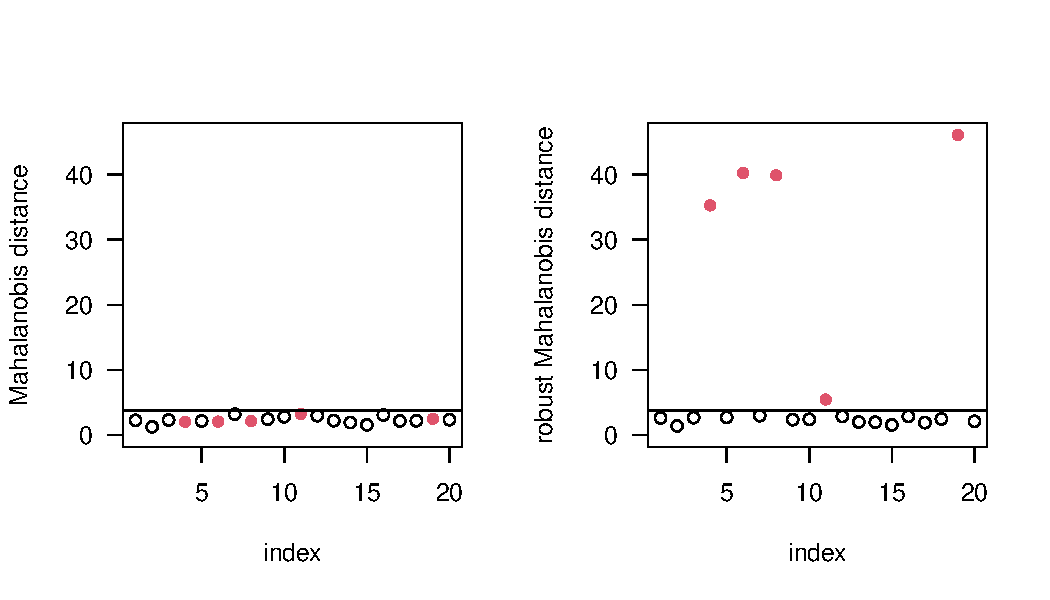
\includegraphics{ICS-009}
\caption{Mahalanobis distance plots for the \code{wood} data set. The red points are according to the robust Mahalanobis distances outliers.}
\label{Maha_wood}
\end{center}
\end{figure}

As can be seen from Figure~\ref{Maha_wood}, the classical Mahalanobis distances do not
reveal any outlier whereas the robust distances classify 4 points as clear outliers
and one borderline case.

The difference between the two Mahalanobis distances can also be observed in a distance versus distance plot, which ideally should
have all points on the bisector. The results of the following code are given in Figure~\ref{Dist_Dist_wood}.
\begin{Schunk}
\begin{Sinput}
R> plot(maha1.wood, maha2.wood, xlab = "regular Mahalanobis distance",
+    ylab = "robust Mahalanobis distance", ylim = c(0, max.maha.wood),
+    xlim = c(0, max.maha.wood), col = out.id + 1, pch = 15 * out.id + 1,
+    las = 1)
R> abline(0, 1)
\end{Sinput}
\end{Schunk}

\setkeys{Gin}{width=0.7\textwidth}
\begin{figure}[t]
\begin{center}
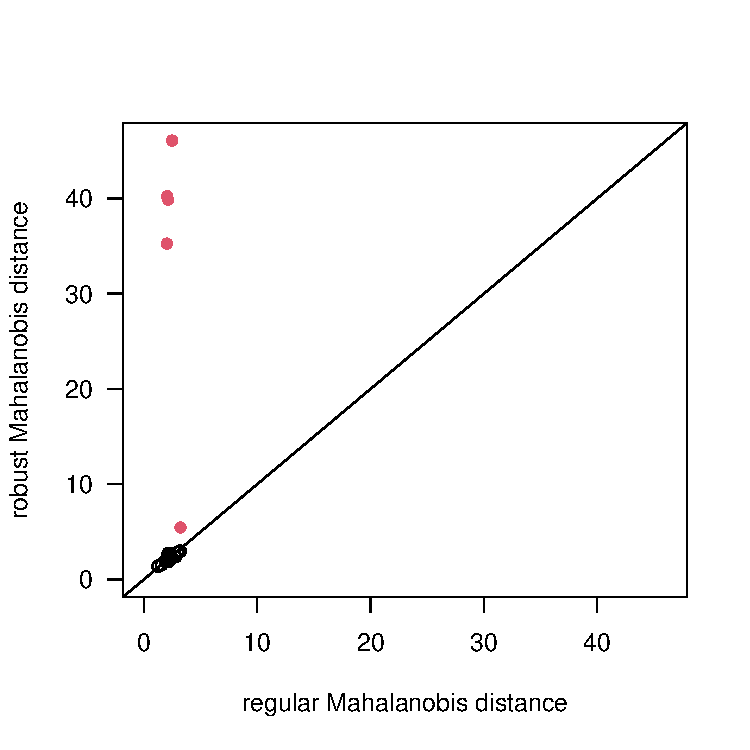
\includegraphics{ICS-011}
\caption{Distance distance plots for the \code{wood} data set. The red points are according to the robust Mahalanobis distances outliers.}
\label{Dist_Dist_wood}
\end{center}
\end{figure}


For outlier identification, it is usually necessary to use Mahalanobis distances based on robust location and scatter statistics.
Although, we still advise using robust scatter statistics for {ICS}, identifying atypical observations using {ICS} tends to be
less dependent on the robustness properties of the scatter matrices being used. As an example, we fit here three different {ICS}
systems based on three different combinations of scatter matrices for the wood data set, and observe that the choice of
$S_1$ and $S_2$ does not seem to greatly affect the results.
\begin{Schunk}
\begin{Sinput}
R> library("ICSNP")
R> my.HR.Mest <- function(X,...) HR.Mest(X,...)$scatter
R> ics.default.wood <- ics(wood)
R> ics.2.wood <- ics(wood, tM(wood)$V, tM(wood, 2)$V)
R> ics.3.wood <- ics(wood, my.HR.Mest, HP1.shape)
R> par(mfrow=c(1, 3), las = 1, mar = c(5, 4, 1, 1) + 0.1)
R> plot(ics.components(ics.default.wood)[,6], xlab = "index", ylab = "IC 6",
+    sub = "ICS using cov and cov4", col = out.id + 1, pch = 15 * out.id + 1)
R> plot(ics.components(ics.2.wood)[,6], xlab = "index", ylab = "IC 6",
+    sub = "ICS using tM(,1) and tM(,2)", col = out.id + 1,
+    pch = 15 * out.id + 1)
R> plot(ics.components(ics.3.wood)[,6], xlab = "index", ylab = "IC 6",
+    sub = "ICS using HR.Mest and HP1.shape", col = out.id + 1,
+    pch = 15 * out.id + 1)
R> par(mfrow = c(1, 1), las = 0)
\end{Sinput}
\end{Schunk}

\setkeys{Gin}{width=\textwidth}
\begin{figure}[t]
\begin{center}
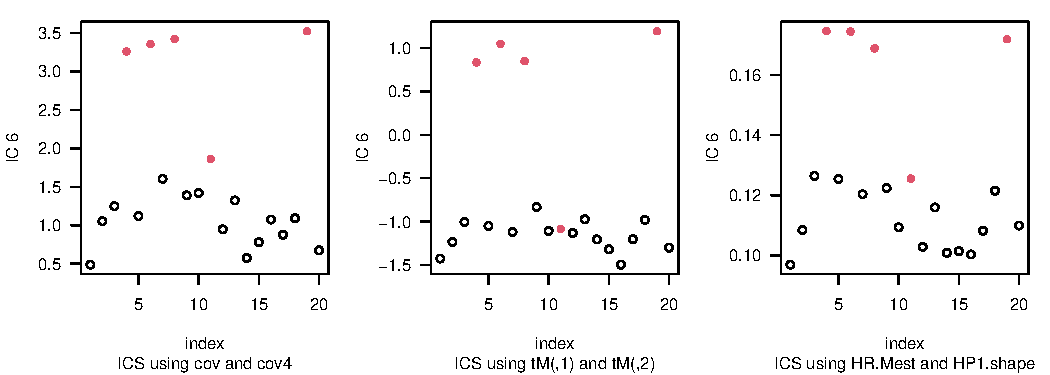
\includegraphics{ICS-013}
\caption{The last invariant coordinate from three different ICS's. The red points are according to the robust Mahalanobis distances outliers.}
\label{ICS_wood}
\end{center}
\end{figure}



From Figure~\ref{ICS_wood}, it can be noted that all three plots clearly display the four extreme points, even though the three pairs of
scatter matrices are quite different. The first {ICS} uses two highly nonrobust scatter matrices, namely they have
unbounded influence functions and zero breakdown points. The other two {ICS} have bounded influence functions, non-zero but not
necessarily high breakdown points. The second {ICS} system presumes first moments, whereas the third does not presume any moments.

The last example also demonstrates the ease of use for the \code{ics} function. One can submit just two function names when the functions return
only the scatter estimates, one can write without difficulties a wrapper around functions that return more than a scatter matrix, as done was
done here for \code{HR.Mest}, or one can submit directly scatter matrices computed in advance, such as (\code{tM(wood)\$V} and
\code{tM(wood, 2)\$V}).

In practice, one often encounters very high dimensional data sets, and so a common practice nowadays is to use {PCA} or
other methods as a dimension reduction technique. The invariant coordinates, i.e., {ICS}, can also be used for this purpose.
We will demonstrate this on Fisher's Iris data set \citep{Fisher1936}.

We start by loading the needed packages and call for the 4 explanatory variables in the data set \code{ics}.
\begin{Schunk}
\begin{Sinput}
R> library("ICS")
R> library("MASS")
R> data("iris")
R> iris.ics <- ics(iris[,1:4])
R> plot(iris.ics, col = as.numeric(iris[,5]))
\end{Sinput}
\end{Schunk}

\setkeys{Gin}{width=0.9\textwidth}
\begin{figure}[t]
\begin{center}
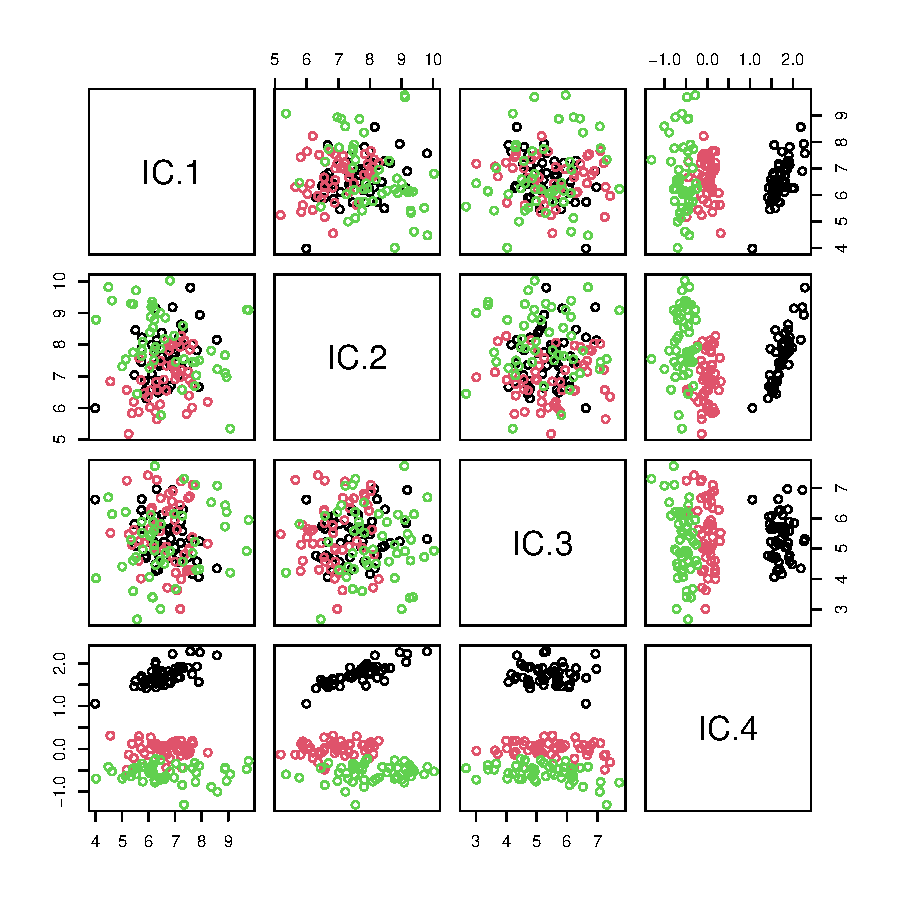
\includegraphics{ICS-015}
\caption{Scatter plot matrix for invariant coordinates of the Iris data set.}
\label{IrisICS}
\end{center}
\end{figure}

The invariant coordinates are then plotted with different colors for the different species in Figure~\ref{IrisICS}.
As can be seen in this figure, the coordinate with the lowest generalized kurtosis separates the three species very
well, even though the species identification is not being taken into account in this analysis. Heuristically spoken one can say that the last
coordinate corresponds to Fisher's linear discriminant subspace.



Since both {ICS} and {PCA} can serve as dimension reduction methods which helps
identify clusters, we also plot for comparison purposes the principal component variables for the Iris data.
\begin{Schunk}
\begin{Sinput}
R> pairs(princomp(iris[,1:4])$scores, col = as.numeric(iris[,5]))
\end{Sinput}
\end{Schunk}

\begin{figure}[t]
\begin{center}
\setkeys{Gin}{width=0.9\textwidth}
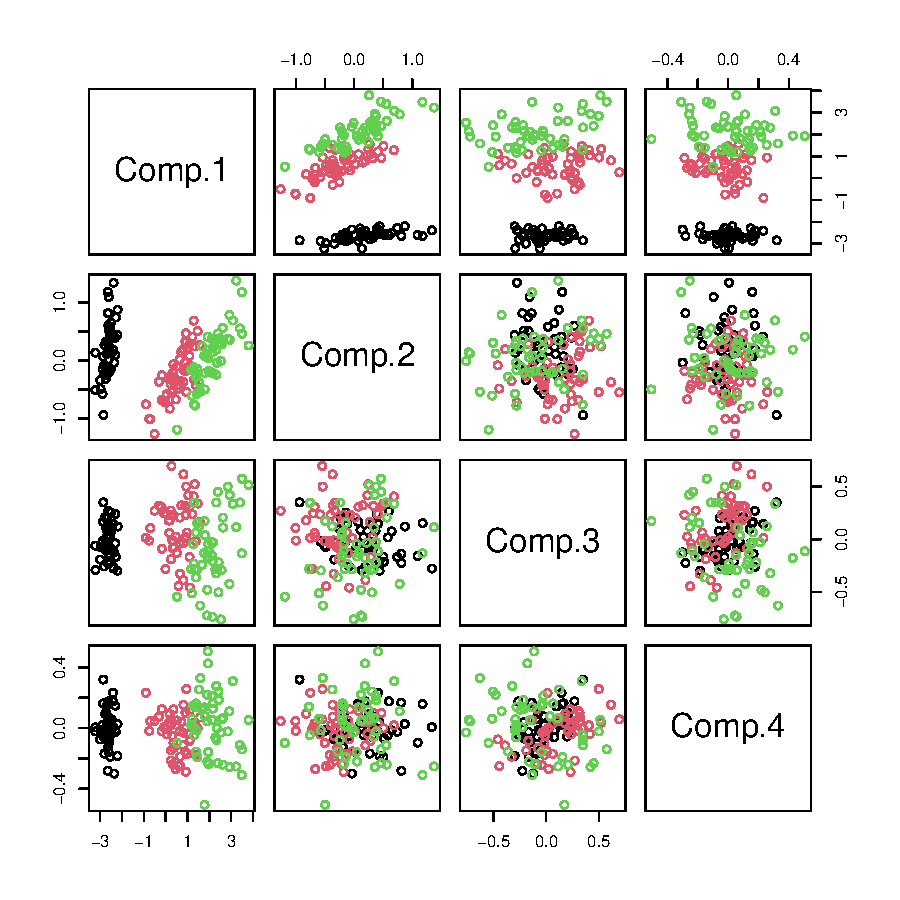
\includegraphics{ICS-017}
\caption{Scatter plot matrix for principal components of the Iris data set.}
\label{IrisPP}
\end{center}
\end{figure}

By comparing Figures~\ref{IrisICS} and \ref{IrisPP}, we note that both plots clearly separates one
species from the other two, but the {PCA} plot is less successful than the {ICS} plot at distinguishing
between the other two species.

Finally, we look at a so called discriminate coordinate plot, which unlike the two previous plots takes into account
the group memberships. Such a plot can be done using \code{ics} by specifying as $S_1$ the regular covariance matrix
and as $S_2$ the within group matrix, which we will call \code{cov.within}.
\begin{Schunk}
\begin{Sinput}
R> p <- dim(iris[, 1:4])[2]
R> n <- dim(iris[, 1:4])[1]
R> ngroup <- aggregate(iris$Species, list(iris$Species), length)$x
R> colMeans.iris <- colMeans(iris[, 1:4])
R> colMeans.iris.groups <- by(iris[, 1:4], iris$Species, colMeans)
R> colMeans.iris.diffs <- sapply(colMeans.iris.groups,"-",
+  colMeans.iris, simplify = FALSE)
R> matrix.iris <- sapply(colMeans.iris.diffs, tcrossprod, simplify = FALSE)
R> freq <- rep(ngroup, each = p^2)
R> matrix.iris <- array(unlist(matrix.iris),
+    dim = c(p, p, nlevels(iris$Species)))
R> cov.within <- rowSums(matrix.iris * freq, dims = 2)/n
R> ics.iris.disc <- ics(iris[,1:4], cov(iris[,1:4]), cov.within)
R> plot(ics.iris.disc, col = as.numeric(iris$Species))
\end{Sinput}
\end{Schunk}

\setkeys{Gin}{width=0.9\textwidth}
\begin{figure}[t]
\begin{center}
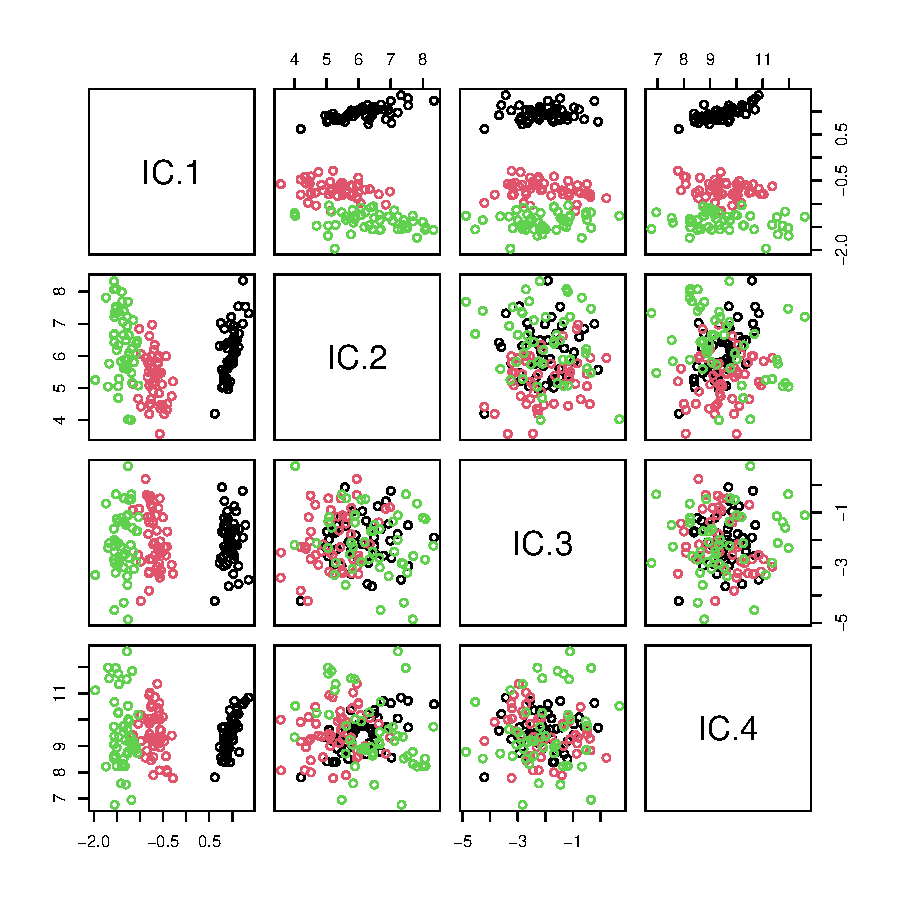
\includegraphics{ICS-019}
\caption{Discriminate coordinate plot for the Iris data set.}
\label{IrisDisc}
\end{center}
\end{figure}


As can be seen from Figures~\ref{IrisICS} and \ref{IrisDisc}, the fourth component of {ICS} a and the first
component of the discriminate analysis are similar.  As noted in Section~\ref{MADdr}, this is what is theoretically
anticipated. We continue by taking a closer look at the 4th invariant coordinate of \code{iris.ics}. Looking at a
kernel density estimate of that component, with rugs representing the different species,
confirms that this component serves very well for discriminating among the three species (see Figure~\ref{Iris_Kernel}).
\begin{Schunk}
\begin{Sinput}
R> iris.z <- ics.components(iris.ics)
R> plot(density(iris.z[,4], bw = 0.15), las = 1,
+  main = "Kernel Density of 4th component")
R> rug(iris.z[1:50, 4], col = 1)
R> rug(iris.z[51:100, 4], col = 2)
R> rug(iris.z[101:150, 4], col = 3, ticksize = -0.03)
\end{Sinput}
\end{Schunk}

\setkeys{Gin}{width=0.7\textwidth}
\begin{figure}[t]
\begin{center}
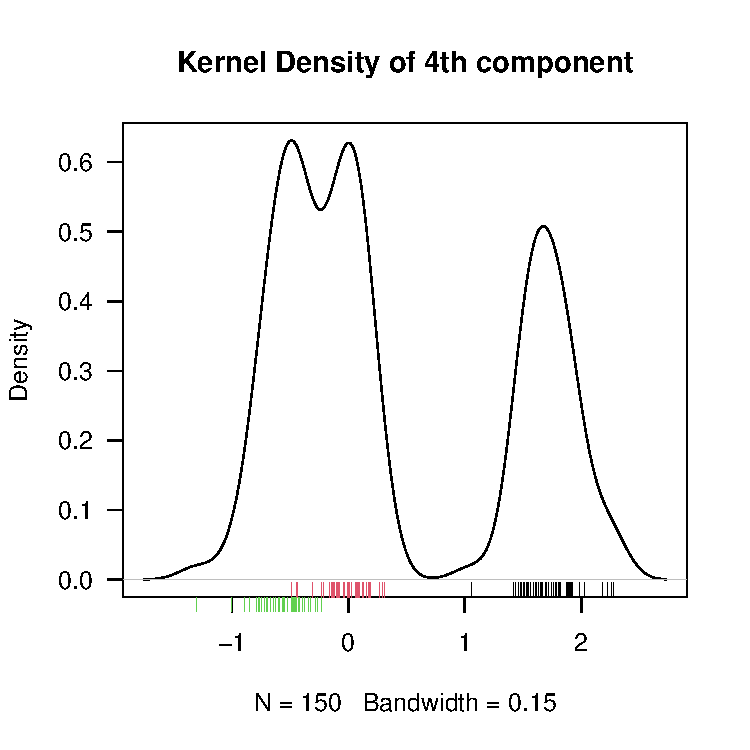
\includegraphics{ICS-021}
\caption{Kernel density estimate of the 4th invariant coordinate of the Iris data set with rugs for the different species. Bandwidth = 0.15.}
\label{Iris_Kernel}
\end{center}
\end{figure}


This result agrees also with \citet{Bugrien2005} who used ICA components for classification for the same data.

To demonstrate this we will randomly select 80\% of the observations of the data set as the training set and use
first the regular data to create a linear discrimination rule to classify the remaining 20\% of the observations and
afterwards we will use the training set to create an invariant coordinate system and use only
the 4th component to create the discrimination rule and classify the test sample using this rule.

\begin{Schunk}
\begin{Sinput}
R> set.seed(4321)
R> train <- sample(1:150, 120)
R> lda.iris <- lda(Species ~ Sepal.Length + Sepal.Width + Petal.Length +
+    Petal.Width, prior = c(1, 1, 1)/3, data = iris, subset = train)
R> table(iris[-train, 5], predict(lda.iris, iris[-train, ])$class)
\end{Sinput}
\begin{Soutput}
             setosa versicolor virginica
  setosa          8          0         0
  versicolor      0         10         1
  virginica       0          1        10
\end{Soutput}
\begin{Sinput}
R> ics.iris <- ics(as.matrix(iris[train, 1:4]))
R> iris.comp4 <- (ics.components(ics.iris))[,4]
R> lda.ics.iris <- lda(iris$Species[train] ~ iris.comp4, prior = c(1, 1, 1)/3)
R> iris.comp4.pred <- (as.matrix(iris[-train, 1:4]) %*% t(coef(ics.iris)))[,4]
R> table(iris[-train, 5], predict( lda.ics.iris, 
+  data.frame(iris.comp4 = iris.comp4.pred))$class)
\end{Sinput}
\begin{Soutput}
             setosa versicolor virginica
  setosa          8          0         0
  versicolor      0         11         0
  virginica       0          0        11
\end{Soutput}
\end{Schunk}

As the two tables show, both methods classify the species pretty well, however using an ICS
we were able to reduce the number of explanatory variables from four to one.

In our analysis of the Iris data, the number of components considered for further analysis has been based only on graphical
arguments. The values of the generalized kurtosis parameters can also be used to help decide which components may be of
further interest. Within the framework of principal axis analysis ({PAA}) clear guidelines have been proposed.
As pointed out in Section~\ref{MADdr}, {PAA} is a special case of {ICS}. Consequently, we demonstrate with the
Iris data how {PAA} can be implemented using the function \code{ics}.

{ICS} yields {PAA} by calling \code{ics} using \code{cov}
and \code{covAxis} for the centered data and requires the absolute
values of the generalized kurtosis measures. Which in this case
correspond to what is called the empirical alignment values in
{PAA}.
\begin{Schunk}
\begin{Sinput}
R> iris.centered <- sweep(iris[,1:4], 2, colMeans(iris[,1:4]), "-")
R> iris.paa <- ics(iris.centered, cov, covAxis, stdKurt = FALSE)
\end{Sinput}
\end{Schunk}

In {PAA}, the generalized kurtosis measures are referred to as the empirical alignment values, which we now
extract.  The mean of the empirical alignment values always equals one.
\begin{Schunk}
\begin{Sinput}
R> emp.align <- iris.paa@gKurt
R> mean(emp.align)
\end{Sinput}
\begin{Soutput}
[1] 1
\end{Soutput}
\begin{Sinput}
R> emp.align
\end{Sinput}
\begin{Soutput}
[1] 1.2336 1.0168 0.9312 0.8184
\end{Soutput}
\end{Schunk}

The {PAA} guidelines given in \citet{Critchley2008} for deciding which components deserve to be considered for
further analysis are those which have an empirical alignment greater than one. This can be visualized by using a
screeplot and checking which components are
indeed larger than one (see Figure~\ref{Iris_PAA}).
\begin{Schunk}
\begin{Sinput}
R> screeplot(iris.paa, las = 1)
R> abline(h = 1)
\end{Sinput}
\end{Schunk}

\setkeys{Gin}{width=0.6\textwidth}
\begin{figure}[t]
\begin{center}
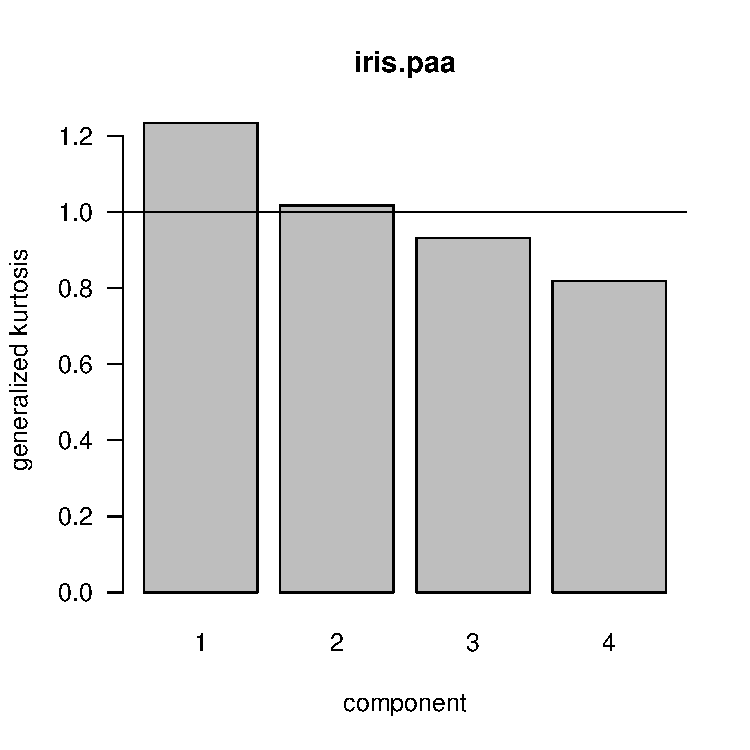
\includegraphics{ICS-026}
\caption{Screeplot for \code{iris.paa}. Components that exceed the vertical line are of interest.}
\label{Iris_PAA}
\end{center}
\end{figure}

So, in this example, we note that the first component is of clear interest whereas the second component may be of
boarderline interest.

\subsection{Independent components analysis}\label{EXics}

Independent components analysis has many applications as, for example, in signal processing or image separation. We will
demonstrate here how the function \code{ics} can be used to restore three images which have been mixed by a random mixing
matrix. The three images, which are displayed in the first row of Figure~\ref{picture_ICA}, are part of the package \pkg{ICS}. Each of
them is on a greyscale and has $130 \times 130$ pixels. The figures are loaded as follows:

\begin{Schunk}
\begin{Sinput}
R> library("ICS")
R> library("pixmap")
R> fig1 <- read.pnm(system.file("pictures/cat.pgm", package = "ICS")[1])
R> fig2 <- read.pnm(system.file("pictures/road.pgm", package ="ICS")[1])
R> fig3 <- read.pnm(system.file("pictures/sheep.pgm", package = "ICS")[1])
\end{Sinput}
\end{Schunk}

For our analysis we have to vectorize the pixel matrices and combine them to form a data set.



\begin{Schunk}
\begin{Sinput}
R> p <- dim(fig1@grey)[2]
R> X <- cbind(as.vector(fig1@grey), as.vector(fig2@grey), as.vector(fig3@grey))
\end{Sinput}
\end{Schunk}

Next, we create a $3 \times 3$ mixing matrix $A$ (the random seed is here set to ensure a proper mixing of the three pictures), mix the
three pictures and use the FOBI algorithm via \code{ics} to recover the pictures.
\begin{Schunk}
\begin{Sinput}
R> set.seed(4321)
R> A <- matrix(rnorm(9), ncol = 3)
R> X.mixed <- X %*% t(A)
R> ICA.fig <- ics(X.mixed, stdB="B")
\end{Sinput}
\end{Schunk}

%% FIXME: Maybe I don't get the point but why do you
%%        have to remove .Random.seed here? Setting the
%%        seed should be sufficinet?!

For a good comparison we plot into one figure in the first row the three original pictures, in the second row the three mixed
pictures, and in the last row the recovered images.

\begin{Schunk}
\begin{Sinput}
R> par(mfrow = c(3, 3), omi = rep(0.1, 4), mai = rep(0.1, 4))
R> plot(fig1)
R> plot(fig2)
R> plot(fig3)
R> plot(pixmapGrey(X.mixed[,1], ncol = p))
R> plot(pixmapGrey(X.mixed[,2], ncol = p))
R> plot(pixmapGrey(X.mixed[,3], ncol = p))
R> plot(pixmapGrey(ics.components(ICA.fig)[,1], ncol = p))
R> plot(pixmapGrey(ics.components(ICA.fig)[,2], ncol = p))
R> plot(pixmapGrey(ics.components(ICA.fig)[,3], ncol = p))
\end{Sinput}
\end{Schunk}

\setkeys{Gin}{width=0.9\textwidth}
\begin{figure}[t!]
\begin{center}
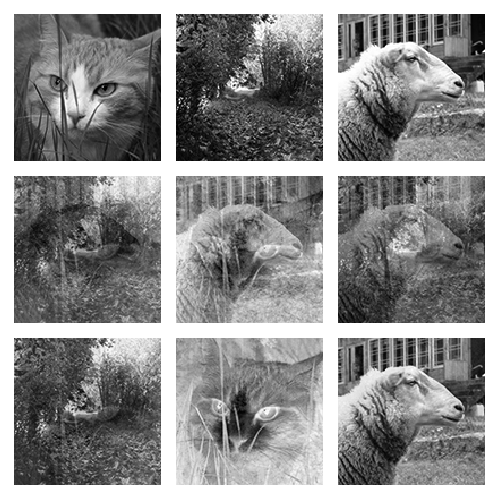
\includegraphics{ICS-pixmap}
\caption{ICA for three pictures. First row are the original pictures, second row the mixed pictures and the last row the by ICA recovered pictures.}
  \label{picture_ICA}
\end{center}
\end{figure}


As Figure~\ref{picture_ICA} shows, we are able to recover the three images quite well. The new order of the images is related
to their generalized kurtosis measures. Also, the cat is now a negative, since the signs of the components are not fixed.
However the positive version of the cat could be easily obtained by multiplying the corresponding component by -1 before the plotting.
%\clearpage

\subsection{Multivariate nonparametrics}\label{EXnp}

In this section, we demonstrate via examples, the use of an invariant coordinate system for estimation and testing problems. For the
estimation example, we choose the componentwise Hodges-Lehmann estimator \citep{HettmanspergerMcKean1998}. For the testing example,
we use the one sample location test using marginal normal scores \citep{PuriSen1971}.

We start the demo with loading the three packages needed.
\begin{Schunk}
\begin{Sinput}
R> library("ICS")
R> library("mvtnorm")
R> library("ICSNP")
\end{Sinput}
\end{Schunk}
Now we will create a simulated data matrix $X$ of 150 samples coming form a $N_{3}((1 \ 2 \ {-1}),I)$ distribution,
a $3 \times 3$ transformation matrix $A$ and a location shift vector $b=(1 \ 1 \ 1)$. The transformed data will be denoted
$X_\mathrm{trans}$. %% FIXME: Or should this be \code{X.trans}?
Also needed is the function \code{HL.estimator} in order to extract the Hodges-Lehmann estimator from the
function \code{wilcox.test}.
\begin{Schunk}
\begin{Sinput}
R> set.seed(2000)
R> X <- rmvnorm(150, c(1, 2,-1))
R> A <- matrix(rnorm(9), ncol = 3)
R> b <- c(1, 1, 1)
R> X.trans <- sweep(X %*% t(A), 1, b, "+")
R> HL.estimator <- function(x){
+  wilcox.test(x, exact = TRUE, conf.int = TRUE)$estimate}
\end{Sinput}
\end{Schunk}

The results when applying then the Hodges-Lehmann estimator on $X$ and transforming the estimate using $A$ and $b$ and
applying the estimator directly on $X_\mathrm{trans}$ differ as the following lines show.
\begin{Schunk}
\begin{Sinput}
R> HLE.X <- apply(X, 2, HL.estimator)
R> as.vector(HLE.X %*% t(A) + b)
\end{Sinput}
\begin{Soutput}
[1]  4.3539 -0.2493 -2.0881
\end{Soutput}
\begin{Sinput}
R> apply(X.trans, 2, HL.estimator)
\end{Sinput}
\begin{Soutput}
[1]  4.3406 -0.2163 -2.0622
\end{Soutput}
\end{Schunk}
since the Hodges-Lehmann estimator is not affine equivariant.

This can be avoided as explained in Section~\ref{MADnp} by using an ICS. We therefore use the function \code{ics}
and choose as $S_1$ the regular covariance matrix and as $S_2$ Tyler's shape matrix. First we will apply it only on $X$, estimate using the obtained
coordinates the Hodges-Lehmann estimate and transform
the estimate back into the original coordinates using the inverse of the transformation matrix $B^{-1}$, this estimate is denoted as \code{HL.ics.X}.
Repeating the same procedure on the transformed data $XA^\top$ we can see that the corresponding estimate \code{HL.ics.AX}
equals the transformed estimate of \code{HL.ics.X}.

\begin{Schunk}
\begin{Sinput}
R> ics.X <- ics(X, S1 = cov, S2 = tyler.shape)
R> HL.ics.Z1 <- apply(ics.components(ics.X), 2, HL.estimator)
R> HL.ics.X <- as.vector(HL.ics.Z1 %*% t(solve(coef(ics.X))))
R> ics.X.trans <- ics(X.trans, S1 = cov, S2 = tyler.shape)
R> HL.ics.Z2 <- apply(ics.components(ics.X.trans), 2, HL.estimator)
R> HL.ics.X.trans <- as.vector(HL.ics.Z2 %*% t(solve(coef(ics.X.trans))))
R> as.vector(HL.ics.X %*% t(A) +b)
\end{Sinput}
\begin{Soutput}
[1]  4.3415 -0.2195 -2.0283
\end{Soutput}
\begin{Sinput}
R> HL.ics.X.trans
\end{Sinput}
\begin{Soutput}
[1]  4.3415 -0.2195 -2.0283
\end{Soutput}
\end{Schunk}
For the testing example we first generate a random sample of size 60 coming from a 4-variate $t_6$ distribution having mean $(0 \ 0 \ 0 \ 0.48)$.
The $4 \times 4$ transformation matrix in this context is called $A2$.
\begin{Schunk}
\begin{Sinput}
R> set.seed(1)
R> Y <- rmvt(60, diag(4), df = 6) + matrix(rep(c(0, 0.48), c(3*60, 60)),
+    ncol = 4)
R> A2 <- matrix(rnorm(16), ncol = 4)
\end{Sinput}
\end{Schunk}
We test the null hypothesis that the sample has the origin as its location on the original data $Y$ first, and then
for the transformed data $YA2^\top$. For invariant tests, the decisions are the same.

\begin{Schunk}
\begin{Sinput}
R> rank.ctest(Y, scores = "normal")
\end{Sinput}
\begin{Soutput}
	Marginal One Sample Normal Scores Test

data:  Y
T = 12, df = 4, p-value = 0.02
alternative hypothesis: true location is not equal to c(0,0,0,0)
\end{Soutput}
\begin{Sinput}
R> rank.ctest((Y %*% t(A2)), scores = "normal")
\end{Sinput}
\begin{Soutput}
	Marginal One Sample Normal Scores Test

data:  (Y %*% t(A2))
T = 8.9, df = 4, p-value = 0.06
alternative hypothesis: true location is not equal to c(0,0,0,0)
\end{Soutput}
\end{Schunk}
As expected the decisions differ, they differ even that much, that assuming an $\alpha$-level of 0.05 we would once reject and once fail to reject
the null hypothesis.

Again, using an ICS avoids this problem. However, when testing a location parameter we have a hypothesis for it which should also be used in the computation
of the scatter matrices. Therefore when creating our ICS we use scatter matrices with respect to the origin.
\begin{Schunk}
\begin{Sinput}
R> Z.Y <- as.matrix(ics.components(ics(Y,
+    S1 = covOrigin, S2 = cov4, S2args = list(location = "Origin"))))
R> rank.ctest(Z.Y, scores = "normal")
\end{Sinput}
\begin{Soutput}
	Marginal One Sample Normal Scores Test

data:  Z.Y
T = 12, df = 4, p-value = 0.02
alternative hypothesis: true location is not equal to c(0,0,0,0)
\end{Soutput}
\begin{Sinput}
R> Z.Y.trans <- as.matrix(ics.components(ics(Y %*% t(A2),
+    S1 = covOrigin, S2 = cov4, S2args = list(location = "Origin"))))
R> rank.ctest(Z.Y.trans , scores = "normal")
\end{Sinput}
\begin{Soutput}
	Marginal One Sample Normal Scores Test

data:  Z.Y.trans
T = 12, df = 4, p-value = 0.02
alternative hypothesis: true location is not equal to c(0,0,0,0)
\end{Soutput}
\end{Schunk}

\section*{Acknowledgments}

The authors are very grateful for Uwe Ligges' helpful comments that improved a lot the functionality of the package.
The authors are also grateful for the comments of the editors, associate editor and the two anonymous referees.
The work of Klaus Nordhausen and Hannu Oja was supported by grants from the Academy of Finland. The work of David
Tyler was supported by NSF Grant DMS-0604596.

\begin{thebibliography}{33}
\newcommand{\enquote}[1]{``#1''}
\providecommand{\natexlab}[1]{#1}
\providecommand{\url}[1]{\texttt{#1}}
\providecommand{\urlprefix}{URL }
\expandafter\ifx\csname urlstyle\endcsname\relax
  \providecommand{\doi}[1]{doi:\discretionary{}{}{}#1}\else
  \providecommand{\doi}{doi:\discretionary{}{}{}\begingroup
  \urlstyle{rm}\Url}\fi
\providecommand{\eprint}[2][]{\url{#2}}

\bibitem[{Bickel(1965)}]{Bickel1965}
Bickel PJ (1965).
\newblock \enquote{On Some Asymptotically Nonparametric Competitors of
  Hotelling's T2.}
\newblock \emph{Annals of Mathematical Statistics}, \textbf{36}, 160--173.

\bibitem[{Bivand \emph{et~al.}(2008)Bivand, Leisch, and
  M{\"a}chler}]{pixmap2008}
Bivand R, Leisch F, M{\"a}chler M (2008).
\newblock \emph{\pkg{pixmap}: Bitmap Images (``Pixel Maps'')}.
\newblock \proglang{R}~package version~0.4-9,
  \urlprefix\url{http://CRAN.R-project.org/package=pixmap}.

\bibitem[{Bugrien(2005)}]{Bugrien2005}
Bugrien JB (2005).
\newblock \emph{Robust Approaches to Clustering Based on Density Estimation and
  Projection}.
\newblock Ph.D. thesis, University of Leeds.

\bibitem[{Cardoso(1989)}]{Cardoso1989}
Cardoso JF (1989).
\newblock \enquote{Source Separation Using Higher Order Moments.}
\newblock In \enquote{Proceedings of IEEE International Conference on
  Accoustics, Speech and Signal Processing,} pp. 2109--2112. Glasgow.

\bibitem[{Caussinus and Ruiz-Gazen(1994)}]{Ruiz-Gazen1994}
Caussinus H, Ruiz-Gazen A (1994).
\newblock \enquote{Projection Pursuit and Generalized Principal Component
  Analysis.}
\newblock In S~Morgenthaler, E~Ronchetti, WA~Stahel (eds.), \enquote{New
  Directions in Statistical Data Analysis and Robustness,} pp. 35--46.
  Birkh{\"a}user Verlag, Basel.

\bibitem[{Chakraborty and Chaudhuri(1996)}]{ChakrabortyChaudhuri1996}
Chakraborty B, Chaudhuri P (1996).
\newblock \enquote{On a Transformation and Re-Transformation Technique for
  Constructing Affine Equivariant Multivariate Median.}
\newblock In \enquote{Proceedings of the American Mathematical Society,} volume
  124, pp. 2539--2547.

\bibitem[{Chakraborty and Chaudhuri(1998)}]{ChakrabortyChaudhuri1998b}
Chakraborty B, Chaudhuri P (1998).
\newblock \enquote{On an Adaptive Transformation and Retransformation Estimate
  of Multivariate Location.}
\newblock \emph{Journal of the Royal Statistical Society, Series B},
  \textbf{60}, 145--157.

\bibitem[{Chakraborty \emph{et~al.}(1998)Chakraborty, Chaudhuri, and
  Oja}]{ChakrabortyChaudhuri1998}
Chakraborty B, Chaudhuri P, Oja H (1998).
\newblock \enquote{Operating Transformation Retransformation on Spatial Median
  and Angle Test.}
\newblock \emph{Statistica Sinica}, \textbf{8}, 767--784.

\bibitem[{Critchley \emph{et~al.}(2008)Critchley, Pires, and
  Amado}]{Critchley2008}
Critchley F, Pires A, Amado C (2008).
\newblock \enquote{Principal Axis Analysis.}
\newblock Unpublished Manuscript.

\bibitem[{D{\"u}mbgen(1998)}]{Dumbgen1998}
D{\"u}mbgen L (1998).
\newblock \enquote{On {T}yler's {$M$}-Functional of Scatter in High Dimension.}
\newblock \emph{Annals of the Institute of Statistical Mathematics},
  \textbf{50}, 471--491.

\bibitem[{Fisher(1936)}]{Fisher1936}
Fisher RA (1936).
\newblock \enquote{The Use of Multiple Measurements in Taxonomic Problems.}
\newblock \emph{Annals of Eugenics}, \textbf{7}, 179--188.

\bibitem[{Genz \emph{et~al.}(2008)Genz, Bretz, and Hothorn}]{mvtnorm2008}
Genz A, Bretz F, Hothorn T (2008).
\newblock \emph{\pkg{mvtnorm}: Multivariate Normal and $t$~Distribution}.
\newblock \proglang{R}~package version~0.9-2,
  \urlprefix\url{http://CRAN.R-project.org/package=mvtnorm}.

\bibitem[{Hettmansperger and McKean(1998)}]{HettmanspergerMcKean1998}
Hettmansperger TP, McKean JW (1998).
\newblock \emph{Robust Nonparametric Statistical Methods}.
\newblock Arnold, London, UK.

\bibitem[{Hyv{\"a}rinen \emph{et~al.}(2001)Hyv{\"a}rinen, Karhunen, and
  Oja}]{HyvarinenKarhunenOja2001}
Hyv{\"a}rinen A, Karhunen J, Oja E (2001).
\newblock \emph{Independent Component Analysis}.
\newblock John Wiley \& Sons, New York, USA.

\bibitem[{Kankainen \emph{et~al.}(2007)Kankainen, Taskinen, and
  Oja}]{KankainenTaskinenOja2007}
Kankainen A, Taskinen S, Oja H (2007).
\newblock \enquote{Tests of Multinormality Based on Location Vectors and
  Scatter Matrices.}
\newblock \emph{Statistical Methods \& Applications}, \textbf{16}, 357--379.

\bibitem[{Kent and Tyler(1991)}]{KentTyler1991}
Kent JT, Tyler DE (1991).
\newblock \enquote{Redescending {$M$}-Estimates of Multivariate Location and
  Scatter.}
\newblock \emph{The Annals of Statistics}, \textbf{19}, 2102--2119.

\bibitem[{M{\"a}chler \emph{et~al.}(2008)M{\"a}chler, Rousseeuw, Croux,
  Todorov, Ruckstuhl, and Salibian-Barrera}]{robustbase2008}
M{\"a}chler M, Rousseeuw P, Croux C, Todorov V, Ruckstuhl A, Salibian-Barrera M
  (2008).
\newblock \emph{\pkg{robustbase}: Basic Robust Statistics}.
\newblock \proglang{R}~package version~0.4-3,
  \urlprefix\url{http://CRAN.R-project.org/package=robustbase}.

\bibitem[{Maronna \emph{et~al.}(2006)Maronna, Martin, and
  Yohai}]{MaronnaMartinYohai2006}
Maronna RA, Martin RD, Yohai VJ (2006).
\newblock \emph{Robust Statistics - Theory and Methods}.
\newblock John Wiley \& Sons, Chichester, UK.

\bibitem[{Nordhausen \emph{et~al.}(2008{\natexlab{a}})Nordhausen, Oja, and
  Ollila}]{NordhausenOjaOllila2008}
Nordhausen K, Oja H, Ollila E (2008{\natexlab{a}}).
\newblock \enquote{Robust Independent Component Analysis Based on Two Scatter
  Matrices.}
\newblock \emph{Austrian Journal of Statistics}, \textbf{37}, 91--100.

\bibitem[{Nordhausen \emph{et~al.}(2008{\natexlab{b}})Nordhausen, Oja, and
  Paindaveine}]{NordhausenOjaPaindaveine2008}
Nordhausen K, Oja H, Paindaveine D (2008{\natexlab{b}}).
\newblock \enquote{Signed-Rank Tests for Location in the Symmetric Independent
  Component Model.}
\newblock \emph{Journal of Multivariate Analysis}.
\newblock \doi{10.1016/j.jmva.2008.08.004}.

\bibitem[{Nordhausen \emph{et~al.}(2006)Nordhausen, Oja, and
  Tyler}]{NordhausenOjaTyler2006}
Nordhausen K, Oja H, Tyler DE (2006).
\newblock \enquote{On the Efficiency of Invariant Multivariate Sign and Rank
  Test.}
\newblock In EP~Liski, J~Isotalo, J~Niemel{\"a}, S~Puntanen, GPH Styan (eds.),
  \enquote{Festschrift for Tarmo Pukkila on his 60th Birthday,} pp. 217--231.
  University of Tampere, Tampere, Finland.

\bibitem[{Nordhausen \emph{et~al.}(2008{\natexlab{c}})Nordhausen, Oja, and
  Tyler}]{NordhausenOjaTyler2008}
Nordhausen K, Oja H, Tyler DE (2008{\natexlab{c}}).
\newblock \enquote{Tools for Exploring Multivariate Data: The Package
  \pkg{ICS}.}
\newblock \emph{Journal of Statistical Software}, \textbf{28}(6), 1--31.
\newblock \urlprefix\url{http://www.jstatsoft.org/v28/i06/}.

\bibitem[{Nordhausen \emph{et~al.}(2007)Nordhausen, Sirki{\"a}, Oja, and
  Tyler}]{ICSNP2007}
Nordhausen K, Sirki{\"a} S, Oja H, Tyler DE (2007).
\newblock \emph{\pkg{ICSNP}: Tools for Multivariate Nonparametrics}.
\newblock \proglang{R}~package version~1.0-2,
  \urlprefix\url{http://CRAN.R-project.org/package=ICSNP}.

\bibitem[{Oja \emph{et~al.}(2006)Oja, Sirki{\"a}, and
  Eriksson}]{OjaSirkiaEriksson2006}
Oja H, Sirki{\"a} S, Eriksson J (2006).
\newblock \enquote{Scatter Matrices and Independent Component Analysis.}
\newblock \emph{Austrian Journal of Statistics}, \textbf{35}, 175--189.

\bibitem[{Puri and Sen(1971)}]{PuriSen1971}
Puri ML, Sen PK (1971).
\newblock \emph{Nonparametric Methods in Multivariate Analysis}.
\newblock John Wiley \& Sons, New York, USA.

\bibitem[{{\proglang{R} Development Core Team}(2008)}]{R272}
{\proglang{R} Development Core Team} (2008).
\newblock \emph{\proglang{R}: A Language and Environment for Statistical
  Computing}.
\newblock \proglang{R} Foundation for Statistical Computing, Vienna, Austria.
\newblock {ISBN} 3-900051-07-0, \urlprefix\url{http://www.R-project.org/}.

\bibitem[{Rousseeuw and van Driessen(1999)}]{RousvanDri1999}
Rousseeuw PJ, van Driessen K (1999).
\newblock \enquote{A Fast Algorithm for the Minimum Covariance Determinant
  Estimator.}
\newblock \emph{Technometrics}, \textbf{41}, 212--223.

\bibitem[{Rousseeuw and van Zomeren(1990)}]{RousvanZom1990}
Rousseeuw PJ, van Zomeren BC (1990).
\newblock \enquote{Unmasking Multivariate Outliers and Leverage Points.}
\newblock \emph{Journal of the American Statistical Association}, \textbf{85},
  633--639.

\bibitem[{Todorov(2008)}]{rrcov}
Todorov V (2008).
\newblock \emph{\pkg{rrcov}: Scalable Robust Estimators with High Breakdown
  Point}.
\newblock \proglang{R}~package version~0.4-07,
  \urlprefix\url{http://CRAN.R-project.org/package=rrcov}.

\bibitem[{Tyler(1987)}]{Tyler1987}
Tyler DE (1987).
\newblock \enquote{A Distribution-Free {$M$}-Estimator of Multivariate
  Scatter.}
\newblock \emph{The Annals of Statistics}, \textbf{15}, 234--251.

\bibitem[{Tyler \emph{et~al.}(2008)Tyler, Critchley, D{\"u}mbgen, and
  Oja}]{Tyler2008}
Tyler DE, Critchley F, D{\"u}mbgen L, Oja H (2008).
\newblock \enquote{Exploring Multivariate Data via Multiple Scatter Matrices.}
\newblock \emph{Journal of the Royal Statistical Society, Series B}.
\newblock Accepted.

\bibitem[{Venables and Ripley(2002)}]{MASS2002}
Venables WN, Ripley BD (2002).
\newblock \emph{Modern Applied Statistics with \proglang{S}}.
\newblock Springer-Verlag, New York, fourth edition.

\bibitem[{Wang \emph{et~al.}(2003)Wang, Raftery, and Fraley}]{covRobust}
Wang N, Raftery A, Fraley C (2003).
\newblock \emph{\pkg{covRobust}: Robust Covariance Estimation via Nearest
  Neighbor Cleaning}.
\newblock \proglang{R}~package version~1.0,
  \urlprefix\url{http://CRAN.R-project.org/package=covRobust}.

\end{thebibliography}

\end{document}
